\chapter{General Overview}
\abstract*{General}

\section{Description of Vegvisir Implementation}

The Vegvisir blockchain is used to share information within a group of
participants. The participants are defined prior to creation of the blockchain.
This is also true concerning the type of information that is shared. The set-up
is differs slightly from the instantiation of the database. The fundamental
use of this structure is to ensure that events that happen in a distributed
system are securely logged. The protocol has implications for food supply
tracking, emergency response, food management and much more.

%\begin{figure*}[!htbp]
\begin{wrapfigure}{r}{0.25\textwidth}
    %\centering
    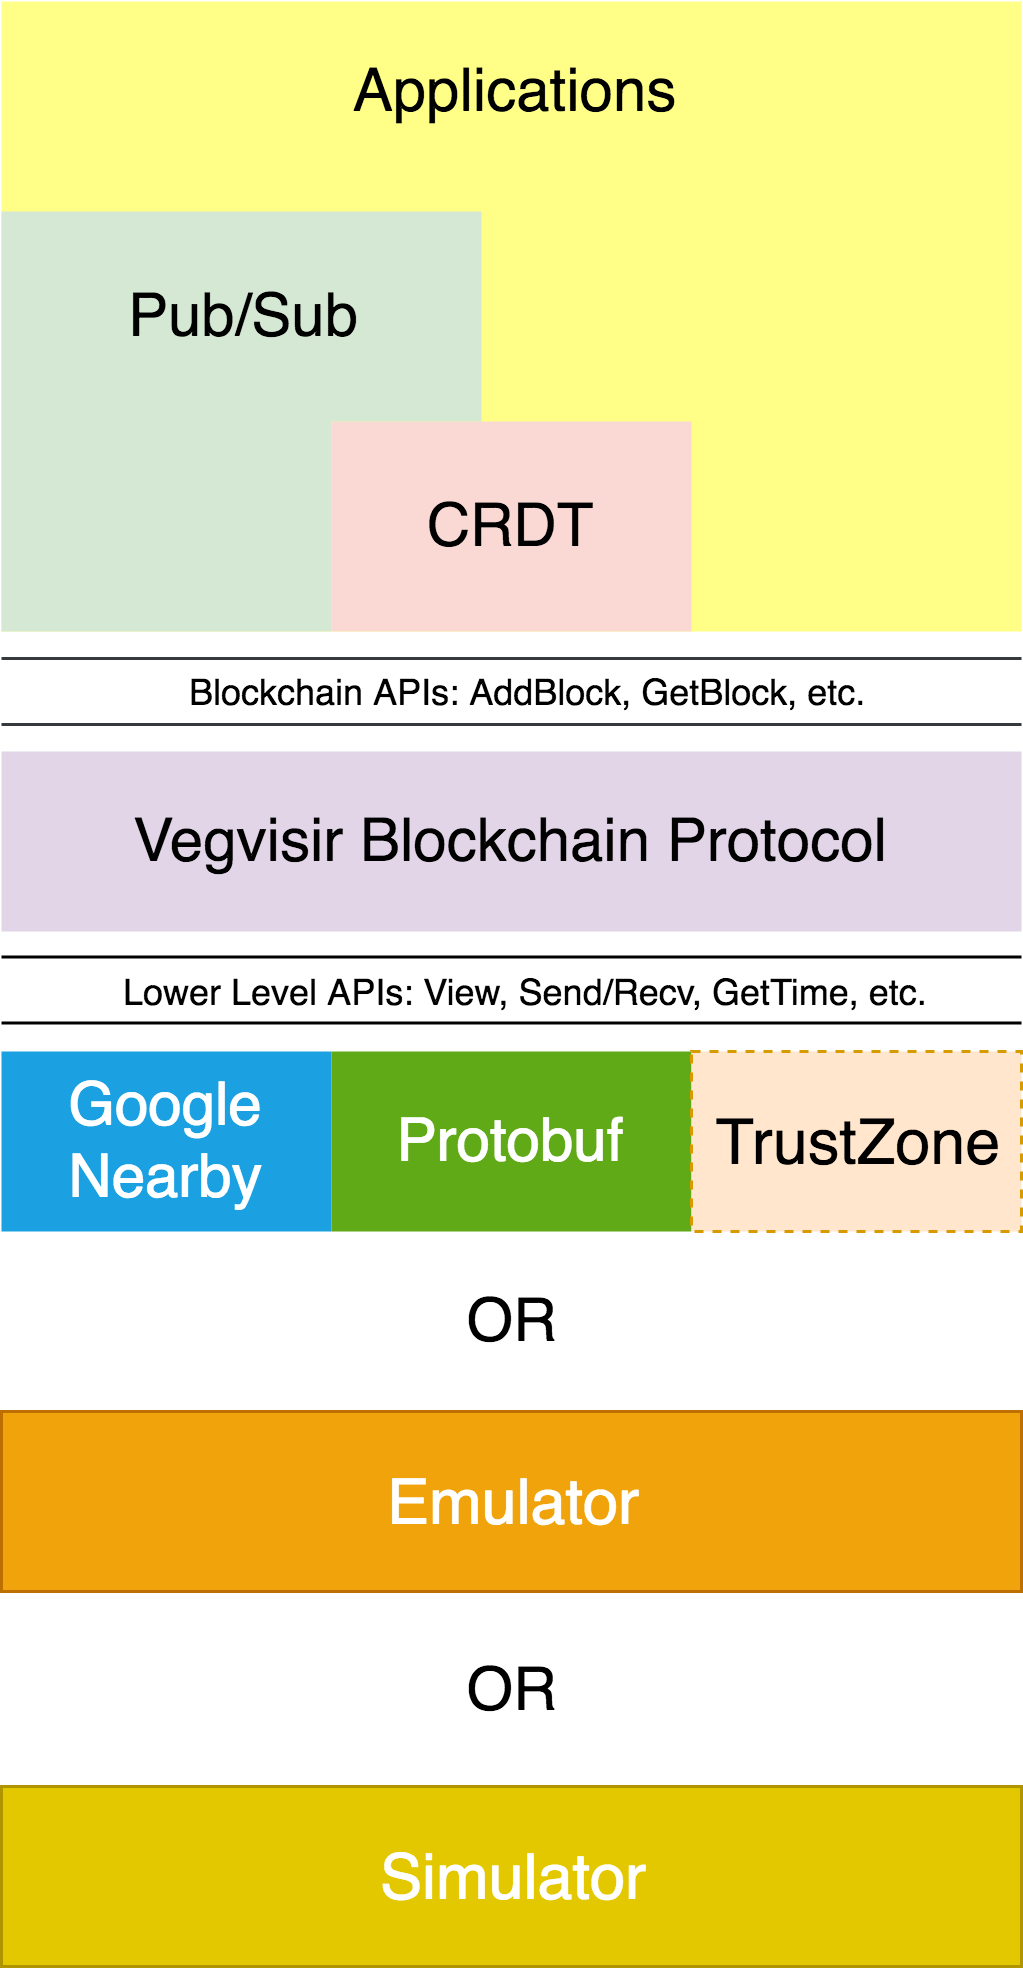
\includegraphics[scale=0.15]{Veg_Structure.png}
    \caption{Vegvisir Structure}
    \label{fig:structure}
\end{wrapfigure}
%\end{figure*}

The implementation can be broken down into three different sections:
\begin{enumerate}
    \item{ Core }
    \item{ Application layer }
    \item{ Lægra }
\end{enumerate}
The figure \ref{fig:structure} shows the overview of the system. The
\emph{core} is listed as "Vegvisir Protocol" in lavender. The application layer
is above it, and Lægra can be represented by Protobuf,
TrustZone, or any of the other included methods.
